\chapter{Project Description}
\label{ch:project_description}

\section{Overview of Ops-Edge}
\label{sec:project_description:overview}
Ops-Edge serves as a dynamic cloud-based solution meticulously designed to revolutionize incident reporting and management across diverse operational environments such as airports, stadiums, and amusement parks. Acting as a centralized hub for coordination, Ops-Edge facilitates seamless collaboration among relevant parties, ensuring swift resolution of incidents to uphold safety and operational efficiency. It also acts as a platform that integrates with external data sources to provide real-time updates and insights, enhancing the overall user experience.

\section{Ops-Edge Architecture}
\label{sec:project_description:opsedge_architecture}

The Ops-Edge Architecture, depicted in Figure~\ref{fig:opsedge_architecture}, provides a high-level overview of a cloud-based application designed to collect, process, and potentially analyze data.

\begin{figure}[h]
    \centering
    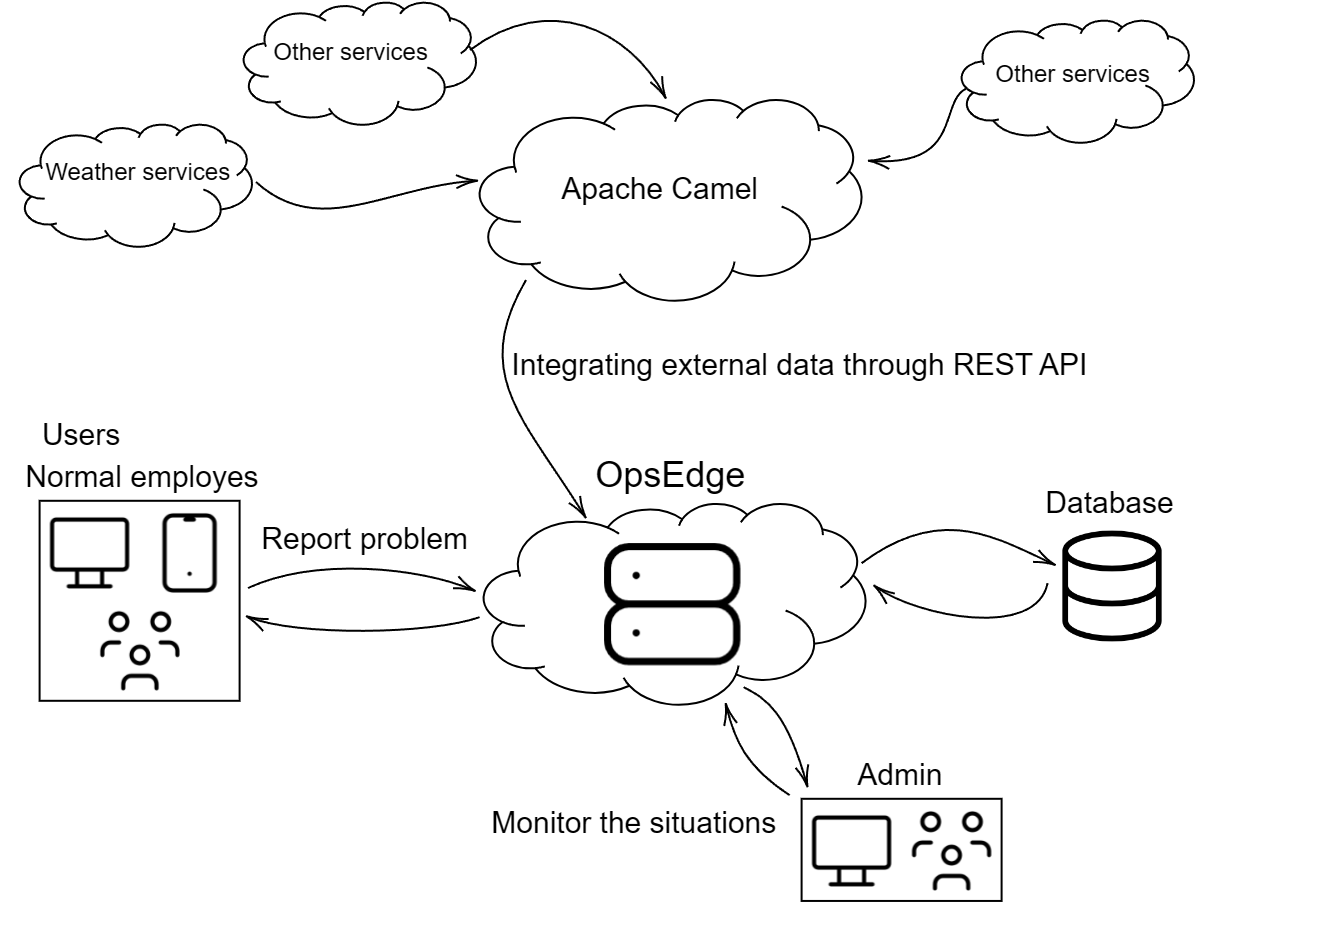
\includegraphics[width=0.9\textwidth]{gfx/opsedge-architecture.png}
    \caption{OpsEdge Architecture}
    \label{fig:opsedge_architecture}
\end{figure}

The architecture is composed of the following components:

\begin{itemize}
    \item \textbf{Users:} This layer represents the various user groups that interact with the application. It can include normal employees who report problems, and administrators who monitor the situations.
    \item \textbf{OpsEdge:} This is the main component of the application. The web application is used to interact with the application, where the users can report problems, monitor the situations, and analyze data.
    \item \textbf{Database:} The database stores all the data collected by the application.
    \item \textbf{Apache Camel:} This is the integration layer of the application. It is responsible for collecting data from various sources, processing it, and giving it to the OpsEdge component through a REST API\@.
    \item \textbf{Services:} These are the various services that the application can use to integrate data with.
\end{itemize}

%
% Section: Project Implementation
%
\section{Project Implementation}
\label{sec:project_description:project_implementation}
There are essentially two main components of the Ops-Edge project: the backend server and the frontend applications. The 3rd component are the integration with external systems and services using \href{https://camel.apache.org/}{Apache Camel} as the integration framework.

\begin{itemize}
    \item \textbf{Backend Server:} The backend server is responsible for processing incoming requests, managing data, and orchestrating communication with the frontend and external data sources. The backend server is built using Python and the Flask framework, with addition of \href{https://flask-appbuilder.readthedocs.io/en/latest/}{Flask-Appbuilder}, which provides a robust foundation for developing web applications. Additionally, the backend server leverages various libraries and tools to enhance its functionality, such as \href{https://www.sqlalchemy.org/}{SQLAlchemy} for database management and \href{https://flask-socketio.readthedocs.io/en/latest/}{Flask-SocketIO} for real-time communication.

    \item \textbf{Frontend Applications:} The frontend applications are the user-facing components of Ops-Edge, providing an intuitive interface for users to interact with the application. The frontend applications are built using React, a popular JavaScript library for building user interfaces. To streamline development and ensure consistency, the frontend applications utilize the Mantine framework, which offers a wide range of components and utilities for building modern web applications. It will also leverage the capabilities of Socket.IO to enable real-time communication with the backend.

    \item \textbf{Integration with External Systems:} Ops-Edge integrates with external systems and services to enhance its functionality and provide a seamless user experience. To facilitate this integration, the project uses Apache Camel, an open-source integration framework that simplifies the process of connecting disparate systems. Apache Camel provides a flexible and extensible platform for defining integration routes, transforming data, and routing messages between systems~\cite{noauthor_home_2024}.
\end{itemize}